% !TEX root =  main.tex



\chapter{Experimental Evaluation}
\label{chap:experimentalevaluation}
\pagestyle{plain}

In this chapter, we conduct a performance evaluation of the implementation, focusing on the following questions:

\begin{itemize}
    \item How compact are the size of the datasets' summaries?
    \item How long does it take to generate the summaries?
    \item How accurate are the query results?
    \item What is the impact of the in-memory LSH-Indexes on startup time?
    \item What is the impact of the optimization algorithm?
\end{itemize}

All tests are performed on a machine running Windows 11 with 16 GB of RAM, and 11th Gen Intel Core i7-1165G7 @ 2.80GHz processor. The LSH indexes are configured with threshold of 0.7 and MinHash size of 128.

\section{Datasets}

The three datasets used are TPC-DI, WikiData, and synthesized Open Data. The first two datasets were provided by Valentine \cite{valentine}, while the third one by \cite{tusZhu}.

TPC-DI ($\sim$35MB) is a synthetic dataset used for data integration benchmark. In \cite{valentine}, the authors created schema matching situations by taking the \textit{Prospect} table from TPC-DI 1.1.0 with a scale factor of three, and split the table in various ways: depending on if the situations were join or union, the table is horizontally or vertically split, with varying degree of overlaps between split instances. In some variants, noises were also added to the instances and schemas, i.e, typos, additional characters added or removed from the table name or a value to differentiate the split versions from each other. For our experiments, we random select 3 split table pairs for each schema matching case presented in the paper: joinable, semantically-joinable, unionable and view-unionable. Each table varies from 11 to 22 columns and 7492 to 14983 rows.

WikiData ($\sim$10MB) is a real world dataset that is used for Wikimedia projects. The authors focused on the table \textit{musicians} in the dataset and manually created split pairs of the table for each matching scenarios. In order to replicate a real-life situation, column names are replaced with synonyms (e.g. partner $\rightarrow$ spouse), and values were change to alternative versions (e.g. Elvis Presley $\rightarrow$ Elvis Aaron Presley). Each table varies from 13 to 20 columns and 5423 to 10846 rows.

The synthesized Open Data dataset from \cite{tusZhu} ($\sim$1,1GB) is used exclusively for union scenario. The tables were generated from a base of 32 tables from Canadian and UK open government data using random projections and selections. Each table ranges from 1 to 40 columns and about 100 to 10000 rows.

\section{Metrics}

Due to varying methodologies in research papers, we employ three metrics to measure the effectiveness of our implementation. The first metric of choice is $Recall@ground\_truth$ from \cite{valentine}:

\[Recall@ground\_truth = \frac{\text{\# of top-k matches}}{\text{k}}\]

where k is the size of the ground truth. This metric is chosen since it shows the ranking's quality of the top relevant results with respect to the ground truth. We use this metric mainly on the first two datasets.

This metric is however not employed in \cite{d3l}, whose implementation we would like to compare with, as it is most similar to ours. There, the system returns ranked matches between tables and not columns. Consequently, the metrics they used: $Precision@k$ and $Recall@k$ are not fully compatible with ours. Nevertheless, we still measure $Precision@k$ and $Recall@k$ on the third dataset (which \cite{d3l} also used) to show that the trends in our diagram as k grows match those in their implementation.

\section{Single Similarity Measure}

First, we compare how each similarity measure fares when being executed in isolation. The result of the experiment performed on the TPC-DI and WikiData datasets is shown in figure \ref{fig:singleMeasure} as a candlestick diagram, depicting the minimum, 1st quartile, 3rd quartile and maximum value of the results. The average results are shown in table \ref{tab:averageRecallSingleMeasure}. Both table name measures that rely on syntactic and semantic similarity perform noticeably worse than other measures, recalling only 7\% to 14\% of matches on average for each matching scenario. This is understandable, as using table name alone to find matches would return all attributes in that table, ignoring the similarities on the column-level. Conversely, the column name measure that uses WordNet for semantic similarity show the highest result, indicating a high correlation between the attribute name and its joinablity/unionability

\begin{table}[ht]
    \centering
    \begin{tabular}{|c|c|}
        \hline
        Measures  & Average \\
        \hline
        Table name WordNet & 0.14 \\
        Column name WordNet & 0.65 \\
        Table name q-gram & 0.07 \\
        Column name q-gram & 0.31 \\
        Values set overlap & 0.48 \\
        Value format overlap & 0.3 \\
        \hline
    \end{tabular}
    \caption{Average $recall@ground\_truth$ of individual measures}
    \label{tab:averageRecallSingleMeasure}
\end{table}

\begin{figure}[ht]
    \centering
    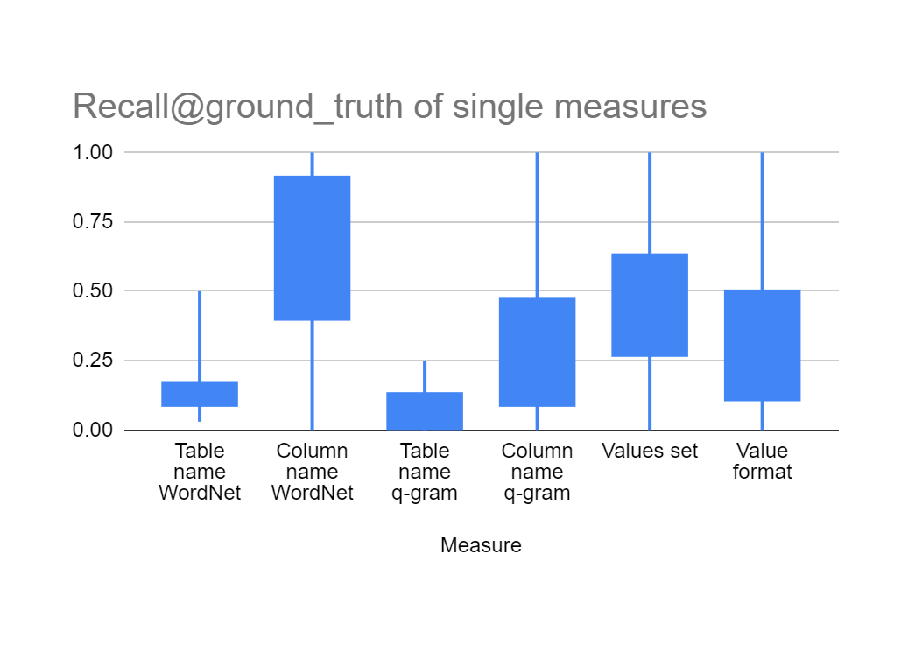
\includegraphics[scale=0.6]{singleMeasure.pdf}
    \caption{Effectiveness of similarity measures when used in isolation}
    \label{fig:singleMeasure}
\end{figure}

\section{Combined Similarity Measure}\label{combinedMeasures}

To evaluate the effectiveness of the similarity measures when aggregated, we measured $Recall@ground\_truth$ on the TPC-DI and WikiData datasets, allowing for comparison with the schema matching techniques in \cite{valentine}. $Precision@k$ and $Recall@k$ were measured on the synthesized Open Data dataset with k ranging from 1 to 400, allowing for comparison with \cite{d3l}. Precision and Recall at each k are the averages computed by perform 20 randomly selected query tables from the dataset. The similarity measures are combined in two different ways: LSH only and mixed:

\begin{itemize}
    \item LSH only: Use only scores from the LSH indexes (table name q-gram, column name q-gram, values set, values format) to aggregate the results.
    \item Mixed: Instead of using table name q-gram and column name q-gram, we use WordNet for table name and column name calculation, while keeping the values set and values format from the LSH indexes like above.
\end{itemize}

Separating the combined measures this way allow us to see whether the additional process of pair-wise semantic WordNet calculation improve the outcomes or not. Additionally, we also want to test if our hypothesized weighted scheme yield better results. Therefore, for each of the two combined measures proposed above, we split the experiment into two weighting schemes: average and weighted average. Average weight means all similarity measures have the same weight when aggregated, while the measures in the weighted average scheme are provided the following weights (table \ref{tab:weights}), which were set up following the intuition from section \ref{measureObject}.

\begin{table}[ht]
    \centering
    \begin{tabular}{|c|c|c|}
         \hline
         & Join mode & Union mode \\
         \hline
         Table name & 0.1 & 0.1\\
         Column name & 0.25 & 0.3 \\
         Values set & 0.4 & 0.2 \\
         Value format & 0.25 & 0.4 \\
         \hline
    \end{tabular}
    \caption{Weighting schema}
    \label{tab:weights}
\end{table}

The results of the experiment on TPC-DI and WikiData can be derived from figure \ref{fig:recallAtGT} and table \ref{tab:averageRecallCommbineMeasure}. We can see that the mixed variants perform on average 11\% to 17\% better than the LSH-only variants, confirming that the semantics indicate higher relatedness than purely syntax. Interestingly, the experiment also showed that the weightings have marginal difference on the outcomes in comparison to the average weighting scheme, performing only slightly better in the LSH-only combinations, and worse in the mixed combinations. This may be explained by the small variance between each weights, making the difference in the contributions of each similarity measure not too pronounced. Therefore, more experiments on different weights should be conducted. Nevertheless, the efficacy of our system falls in line with other schema matching techniques introduced in \cite{valentine}, while running on average much faster (hundreds of milliseconds to a few seconds, in comparison to hundreds of seconds).

\begin{table}[ht]
    \centering
    \begin{tabular}{|c|c|}
        \hline
        Measures  & Average \\
        \hline
        LSH average & 0.51 \\
        LSH weighted & 0.52 \\
        Mixed average & 0.68 \\
        Mixed weighted & 0.63 \\
        \hline
    \end{tabular}
    \caption{Average $recall@ground\_truth$ of combined measures}
    \label{tab:averageRecallCommbineMeasure}
\end{table}

\begin{figure}[ht]
    \centering
    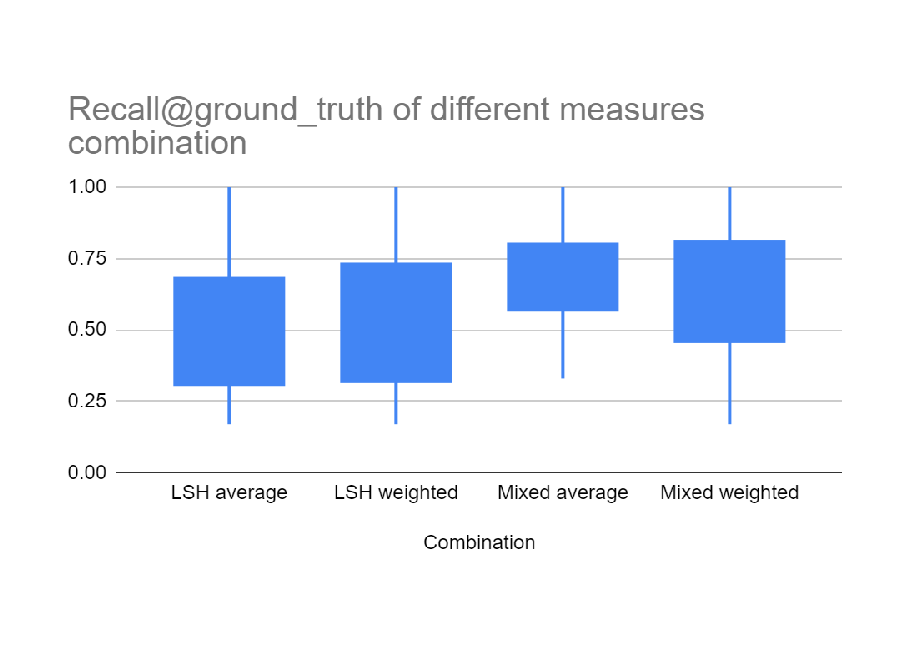
\includegraphics[scale=0.6]{recallAtGT.pdf}
    \caption{Effectiveness of similarity measures when combined}
    \label{fig:recallAtGT}
\end{figure}

As for synthesized Open Data, we show the $Precision@k$ and $Recall@k$ for varying k in figure \ref{fig:precisionAtK} and \ref{fig:recallAtK}, where precision declines linearly from around 0.85 to 0.4 and recall grows from 0.01 to 0.7 as k goes from 1 to 400. Here, the differences between each variant of the combined measures are even less pronounced, ranging from 1\% to 3\%. This also showed that the weights we used for the experiments were not effective in improving accuracy. Still, at k = 50, the system managed to return results with over 0.75 precision, suggesting that the results at the top are mostly relevant matches. Comparing our result with that of \cite{d3l}, their implementation displayed similar trends, but maintained a higher precision at higher k values than ours. This could be due to several factors: 1) they implements dynamic weighting system such that when calculating the score between a query and a candidate, it also considers the score of other candidates to determine if a similarity measure carries strong relatedness signal; 2) The MinHash size used for their LSH indexes were twice as large as ours (256), providing better performance at the cost of additional storage space; 3) Moreover, we also used a variant of Lazo's MinHash sketch that uses a technique called Optimal One-Hash-Permutation \cite{ooph} to reduce sketching time, but also comes with the downside of lower effectiveness.

\begin{figure}[ht]
    \centering
    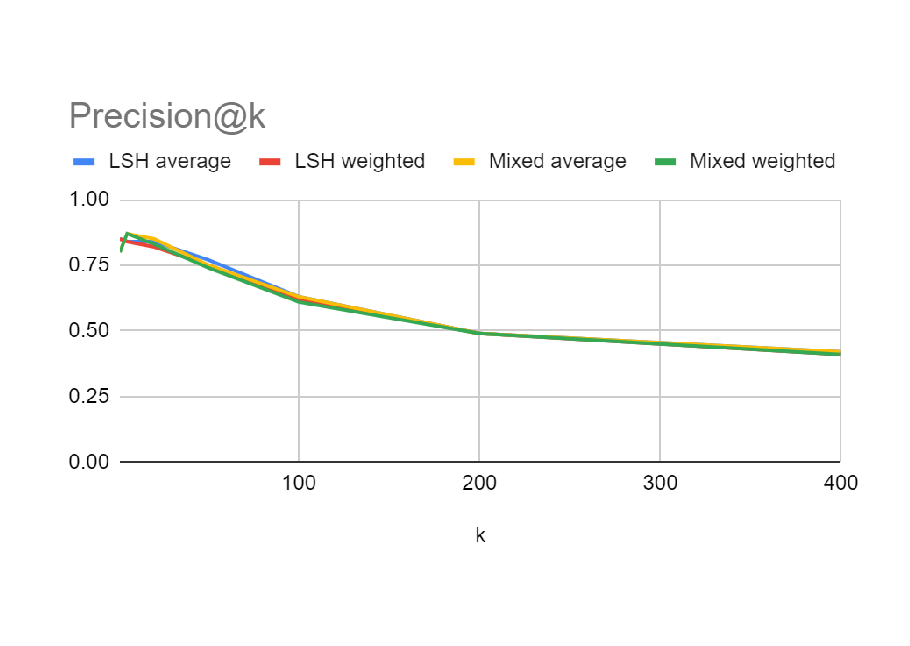
\includegraphics[scale=0.6]{PrecisionAtK.pdf}
    \caption{Precision at various top-k ranking}
    \label{fig:precisionAtK}
\end{figure}

\begin{figure}[ht]
    \centering
    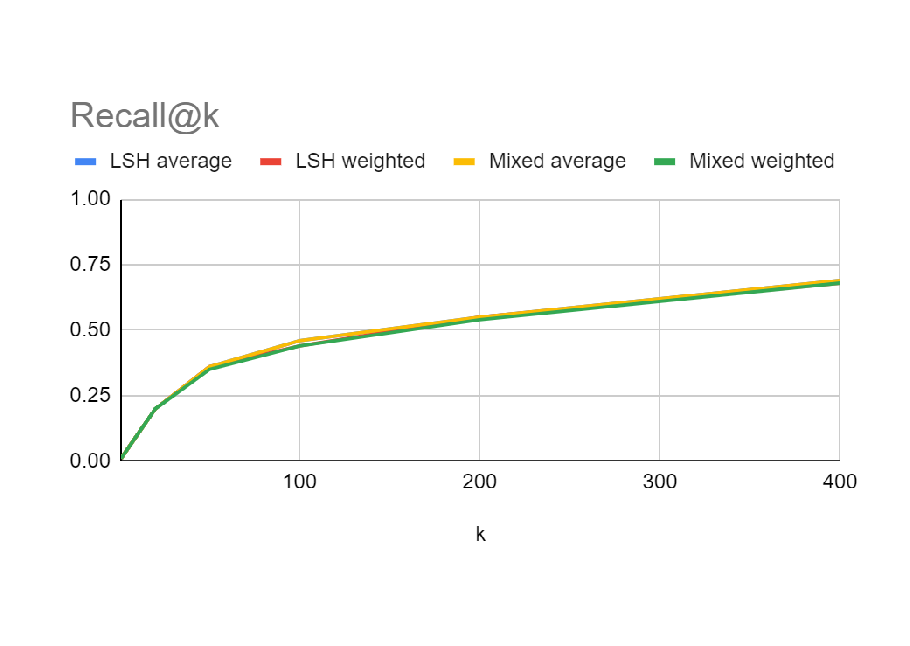
\includegraphics[scale=0.6]{recallAtK.pdf}
    \caption{Recall at various top-k ranking}
    \label{fig:recallAtK}
\end{figure}


\section{Summary Size}\label{summarySizeTest}

To measure the size of the summaries, we divide all of the datasets in 4 sections. The first section contains about 800 columns, the second 3300 columns, the third 5900 columns, and the last 6000 columns. For each sections inserted, we measure the average sketch size (figure \ref{fig:sketchsize}) and the average metadata size (figure \ref{fig:metadatasize}) stored in the database. With each insertion, the average size of the sketches object remain consistent at 6.63kB. This is understandable, as all sketches store the same amount of hash values. Meanwhile, the average size of a metadata object ranges from about 270B to 300B with each iterations. This is due to the fact that the information stored in the metadata is variable: one table name may be very long while other ones are shorter. In total, the metadata and sketches take up about 40MB of storage in the database, meaning the summaries are only 3,55\% of the datasets' original size.

\begin{figure}[ht]
    \centering
    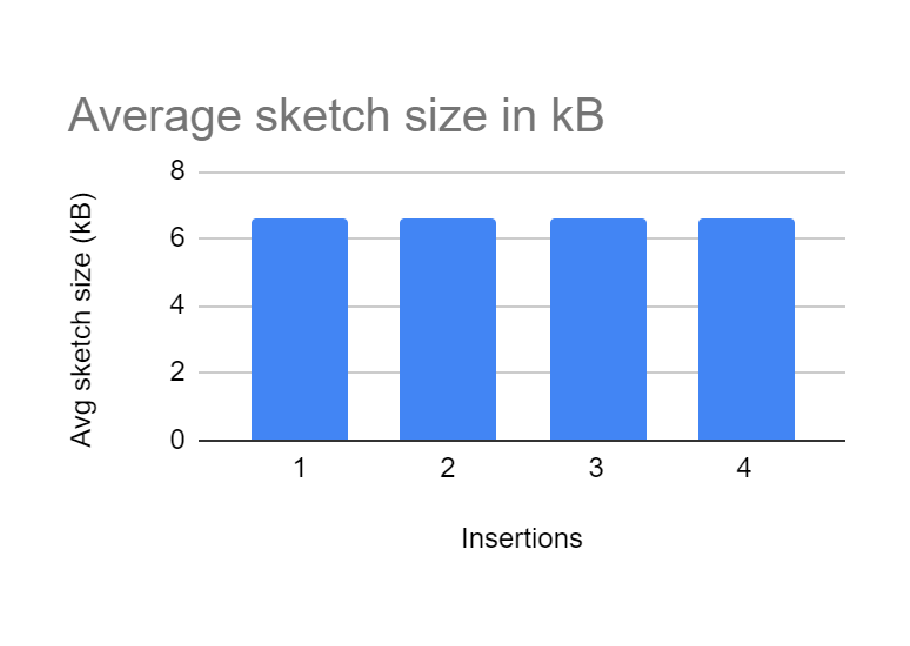
\includegraphics[scale=0.5]{sketchsize.pdf}
    \caption{The average size of the sketches object after each insertions}
    \label{fig:sketchsize}
\end{figure}

\begin{figure}[ht]
    \centering
    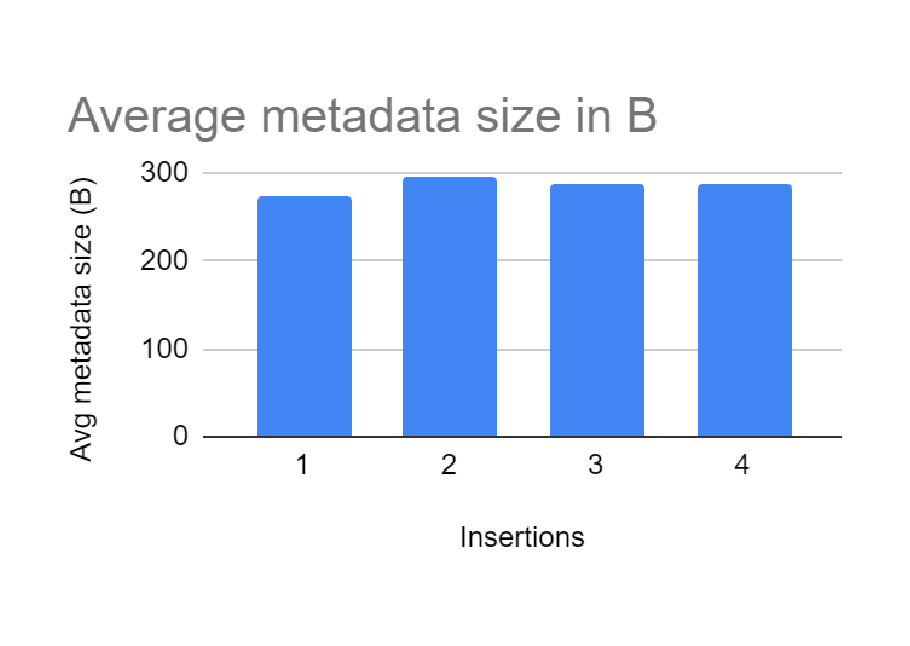
\includegraphics[scale=0.5]{metadatasize.pdf}
    \caption{The average size of the metadata object after each insertions}
    \label{fig:metadatasize}
\end{figure}

\section{Summary Generation Time}

To measure the time it takes to generate summaries, we call the profile() method multiple times on the synthesized Open Data dataset, measuring the time it takes for each types of sketch to be generated, and collect the average runtime. Figure \ref{fig:sketchtime} shows that it took roughly 6 minutes to sketch all columns in the dataset. Most of the time spent were used to generate the values set and the value format, while it took only less than 2 seconds in total for the q-gram sketches of the table name and column name to be generated. Table-wise, it took on average 2 seconds for the profile() method to finish.

\begin{figure}[ht]
    \centering
    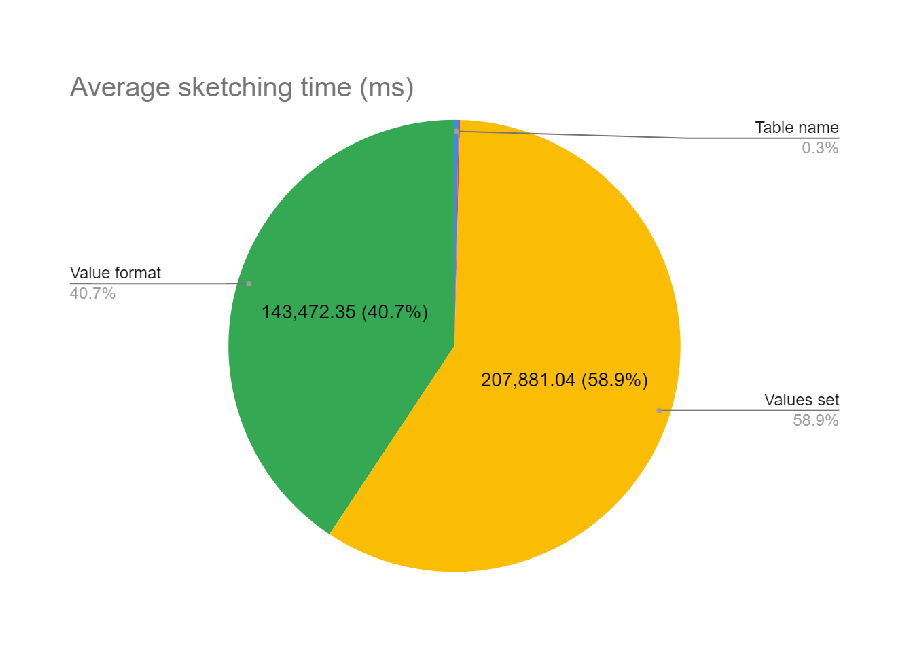
\includegraphics[scale=0.6]{figures/exp1.pdf}
    \caption{Average time taken to sketch the Open Data dataset of 1.1GB}
    \label{fig:sketchtime}
\end{figure}

\section{Effect of in-memory index on startup time}

As mentioned in section \ref{systemArchitecture}, the Lazo's LSH indexes run in main memory. Therefore the sketches need to be loaded from database on startup. We measure the startup time of the system by loading the datasets in 4 sections like in \ref{summarySizeTest}, restarting the server several times for each section loaded, and calculating the average startup time of each iteration. The result is shown in figure \ref{fig:loadIndexTime}, indicating that the startup time grows linearly with the amount of sketches in the database. At the maximum database size containing about 40MB of sketches, the server took roughly 20 seconds to start. As we expect the server to not be restarted often, this time should be negligible.

\begin{figure}[ht]
    \centering
    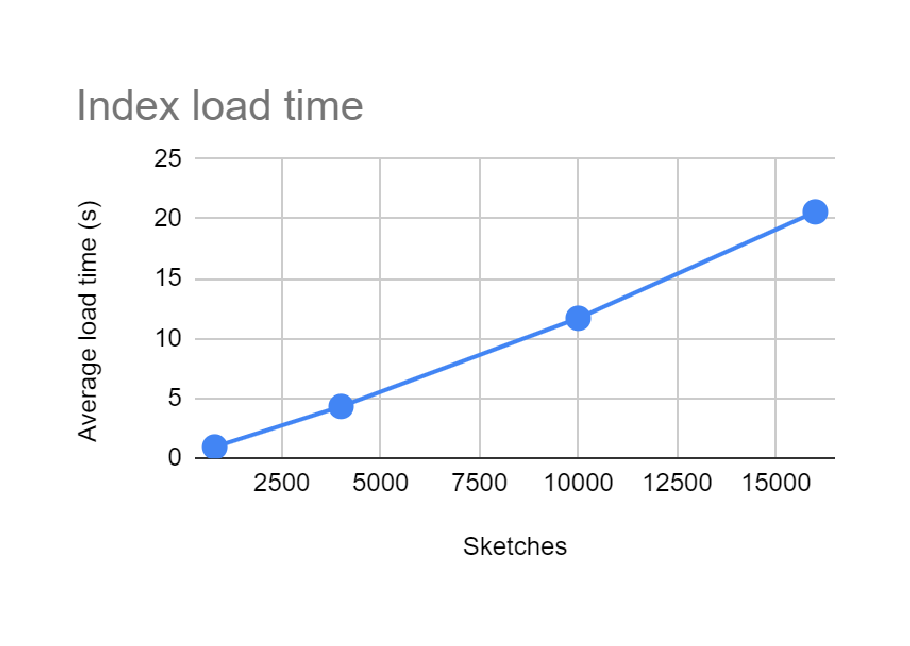
\includegraphics[scale=0.6]{exp2.pdf}
    \caption{Time to startup with increasing amount of sketches}
    \label{fig:loadIndexTime}
\end{figure}

\section{Effect of optimization algorithm}

In this section, we measure the impact of the optimization algorithm \ref{alg:optimization} on the query time. We set up the experiment by first loading all three test datasets into the database, maximizing the amount of candidates that needs to be checked. Then 10 random tables are selected as query, performed at five different query thresholds: 0, 0.2, 0.4, 0.6, 0.8. The similarity measures used are the mixed weighted combinations from \ref{combinedMeasures}. The average runtime at each threshold level is shown in figure \ref{fig:queryThresholdTime}. Without any restriction on the threshold, queries take a long time to calculate. Among our 10 selected queries, there were some that take up to 3 minutes to return. The time reduces on average by 30\% at the 0.4 threshold, and at 0.8 mark, an average query takes only about 10 seconds, which is 6\% of the time taken compared to a 0 threshold. This proves reasonable in practical use cases, as matches with a low similarity score are unlikely to be related anyway.

\begin{figure}[ht]
    \centering
    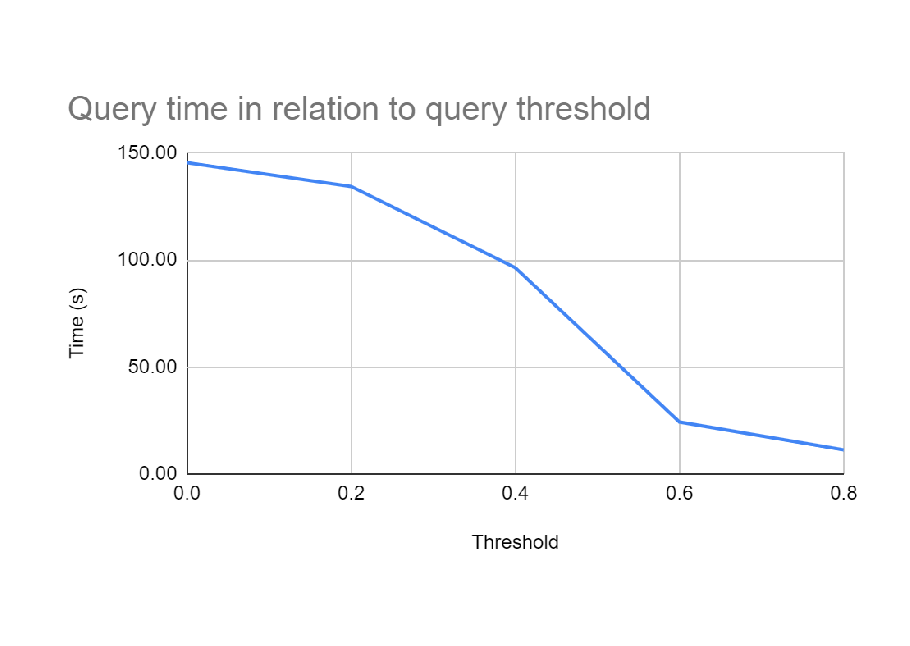
\includegraphics[scale=0.6]{figures/queryThresholdTime.pdf}
    \caption{Query time at various threshold levels}
    \label{fig:queryThresholdTime}
\end{figure}